\section{Choices and parity lifts}\label{sec:parity-lifts}

Fix \(k\ge4\), and let \(t\) and \(T=T_t\) be as in
Section~\ref{sec:wl-tests}. We encode compatible choices by two uncolored
graphs. The comparison will account for every homomorphism into these
graphs, including those whose projections do not describe a choice.

Take a choice system as in Definition~\ref{def:choice}. Form a base graph \(G\) with disjoint vertex sets
\[
 \{(i,d):d\in D_i\}\quad(i\in[t]),\qquad
 \{(h_{ij;\ell},q):q\in L_{ij}\}
 \quad(i<j,\ \ell\notin\{i,j\}).
\]
The first coordinate defines a type map \(\tau:V(G)\to V(T)\).
Its edges are exactly the following, for each permitted \(i,j,\ell\):
\begin{itemize}[nosep]
\item \((i,d)\) and \((j,e)\) are adjacent if
  \(\lambda_{ij}^i(d)=\lambda_{ij}^j(e)\).
\item \((h_{ij;\ell},q)\) is adjacent to \((i,d)\) if
  \(q=\lambda_{ij}^i(d)\), and to \((j,e)\) if
  \(q=\lambda_{ij}^j(e)\).
\item Every \((h_{ij;\ell},q)\) is adjacent to every
  \((\ell,f)\), \(f\in D_\ell\).
\end{itemize}
Thus \(G\) is simple and \(\tau\) is a homomorphism to \(T\).
When evaluating a label map, we identify a vertex in a domain copy
with its underlying domain element. Types and labels are construction
data, not vertex colors supplied to WL. Figure~\ref{fig:helper-incidence}
isolates the two label tests and the unrestricted third incidence.

\begin{figure}[H]
\centering
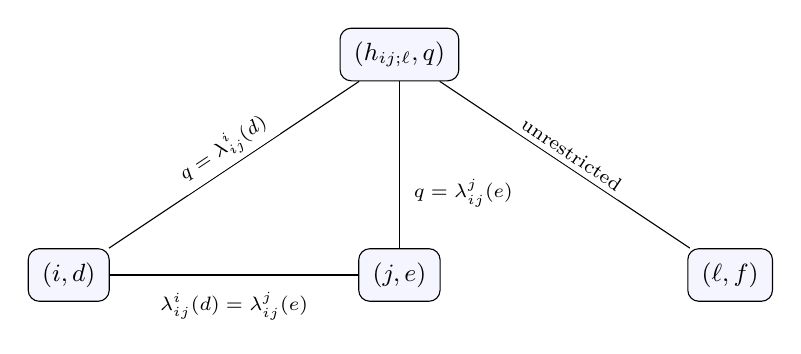
\begin{tikzpicture}[
  vertex/.style={draw,rounded corners,fill=blue!4,inner sep=5pt},
  every node/.style={font=\small},
  test/.style={font=\scriptsize,fill=white,inner sep=2pt}
]
\node[vertex] (left) at (-4.2,0) {\((i,d)\)};
\node[vertex] (middle) at (0,0) {\((j,e)\)};
\node[vertex] (right) at (4.2,0) {\((\ell,f)\)};
\node[vertex] (helper) at (0,2.8) {\((h_{ij;\ell},q)\)};
\draw (helper) -- node[test,sloped,above] {\(q=\lambda_{ij}^i(d)\)} (left);
\draw (helper) -- node[test,pos=.67,right=3pt] {\(q=\lambda_{ij}^j(e)\)} (middle);
\draw (helper) -- node[test,sloped,above] {unrestricted} (right);
\draw (left) -- node[test,below=4pt] {\(\lambda_{ij}^i(d)=\lambda_{ij}^j(e)\)} (middle);
\end{tikzpicture}

\caption{Allowed incidences for one helper in the base graph. The edges
from the helper to types \(i,j\) require its label \(q\) to equal the
corresponding pair label. Its incidence with type \(\ell\) is unrestricted.
The displayed main edge also requires pair-label agreement; other main
edges are omitted. Each labeled point denotes an arbitrary vertex of
its fiber, so an edge is present only when its indicated condition holds.}
\label{fig:helper-incidence}
\end{figure}

Write \(\FF\) for the field with two elements.
\begin{definition}[Parity lifts]\label{def:lifts}
For \(b\in\FF^{V(T)}\), the graph \(X_b\) has vertices
\[
 (u,z),\qquad
 u\in V(G),\quad z\in\FF^{N_T(\tau(u))},\quad
 \sum_{a'\in N_T(\tau(u))}z(a')=b(\tau(u)).
\]
Vertices \((u,z)\) and \((v,w)\) are adjacent precisely when
\(uv\in E(G)\) and \(z(\tau(v))=w(\tau(u))\).
We compare \(X_0\) and \(X_\star:=X_{e_1}\), where
\(e_1(a)=\ind{a=1}\).
\end{definition}

The coordinates of a tag are indexed by neighbor types in \(T\),
including types for which \(u\) has no neighbor in \(G\).
Every type has positive degree. Hence every \(u\) has
\(2^{\deg_T(\tau(u))-1}\) tags for either parity, so both output graphs
have order \(\sum_{u\in V(G)}2^{\deg_T(\tau(u))-1}\).
Both graphs are uncolored and simple: adjacency is symmetric, and a
loop would require a loop in \(G\). The map
\(\pi_b:(u,z)\mapsto u\) is a homomorphism \(X_b\to G\).
If each base fiber has at most \(A\) vertices, Equation~\ref{eq:template-size}
gives the bound \(A M_t\) of Theorem~\ref{thm:choice-reduction}:
the \(t\) main fibers have \(2^{t-2+3\binom{t-1}{2}}\) tags per base vertex,
and the \(3\binom t3\) helper fibers each have four.

The tags on the template itself form Roberson's parity graph
\citep[preprint version, Definition~3.1]{Roberson2026}. Here we additionally remember a
vertex \(u\in G\) whose type matches the tag. Equivalently, if
\(R_b(T)\to T\) is that parity graph's type projection, then \(X_b\)
is the graph on pairs in \(G\times R_b(T)\) with matching projections,
with adjacency in both coordinates. Thus fixing \(\phi:F\to G\)
fixes the template projection \(\tau\phi\). The following proof gives
the resulting local form of Roberson's lift-count comparison and binary
duality~\citep[preprint version, Theorem~3.6 and Lemma~3.8]{Roberson2026}; the compatibility
extraction in Section~\ref{sec:separator} will use the particular
helper structure of our base graph.

\begin{lemma}[Lift counts and their dual obstruction]\label{lem:lift-duality}
For every finite simple graph \(F\),
\(\hom(F,X_0)\ge\hom(F,X_\star)\).
The inequality is strict if and only if there are a homomorphism
\(\phi:F\to G\), vertex weights \(s:V(F)\to\FF\), and edge weights
\(r:E(F)\to\FF\) such that, writing \(a=\tau\circ\phi\),
\begin{equation}\label{eq:dual}
 \begin{aligned}
 \sum_{\substack{y:\,xy\in E(F)\\a(y)=a'}}r(xy)
   &=s(x)
   &&\bigl(x\in V(F),\ a'\in N_T(a(x))\bigr),\\
 \sum_{\substack{x\in V(F)\\a(x)=1}}s(x)&=1.
 \end{aligned}
\end{equation}
Whenever \eqref{eq:dual} holds, the type masses satisfy
\begin{equation}\label{eq:type-mass}
 m_u(A):=\sum_{\substack{x\in A\\a(x)=u}}s(x),
 \qquad
 m_u(V(F))=1
 \quad\bigl(u\in V(T),\ A\subseteq V(F)\bigr).
\end{equation}
All sums of weights are in \(\FF\).
\end{lemma}

\begin{proof}
Fix \(\phi:F\to G\). Its lifts to \(X_b\) correspond to solutions in
variables \(z_{x,a'}\), one for each source vertex \(x\) and each
\(a'\in N_T(a(x))\), of
\[
 \sum_{a'\in N_T(a(x))}z_{x,a'}=b(a(x))
 \quad(x\in V(F)),\qquad
 z_{x,a(y)}+z_{y,a(x)}=0
 \quad(xy\in E(F)).
\]
Indeed a solution gives the map \(x\mapsto(\phi(x),z_x)\), and a lift
uniquely determines these source-indexed vectors.
Equality of projected images does not itself identify these
source-indexed tag variables; all constraints on them are given by
the displayed system.

The coefficient matrix is independent of \(b\). The system for \(b=0\)
has its kernel as solution set; for \(b=e_1\) the solution set is
either empty or a translate of that kernel. Every homomorphism into
\(X_b\) has a unique projection to \(G\), so summing over all \(\phi\)
proves the inequality. Since each homogeneous system is nonempty,
strictness is equivalent to inconsistency of at least one projected
system for \(X_\star\). In particular, contributions from other
projections cannot cancel a strict inequality.

A binary system \(Mz=c\) is inconsistent exactly when some linear
combination of its rows has left side zero and right side one.
For the nontrivial direction, if \(c\notin\operatorname{im}M\), extend
a basis of \(\operatorname{im}M\) by \(c\) to obtain a linear functional
vanishing on \(\operatorname{im}M\) and taking value one at \(c\).
Let \(s(x)\) and \(r(xy)\) be the coefficients of the vertex and edge
equations above. The coefficient of \(z_{x,a'}\) in their combination is
\(s(x)+\sum_{y:\,xy\in E(F),\,a(y)=a'}r(xy)\),
and the right side for \(X_\star\) is \(\sum_{a(x)=1}s(x)\).
This gives exactly \eqref{eq:dual}, without any independence assumption
on the equation rows.

For adjacent types \(u,v\), sum the first equation of
\eqref{eq:dual} over all vertices of type \(u\), using neighbor type
\(v\). The result is the total \(r\)-weight of the edges between these
two types. Summing from type \(v\) gives the same total, so
\(m_u(V(F))=m_v(V(F))\). Since \(T\) is connected and
\(m_1(V(F))=1\), every type mass is one.
\end{proof}

\begin{lemma}[A choice supplies a witness]\label{lem:choice-witness}
A successful choice gives
\(\hom(T,X_0)>\hom(T,X_\star)\), and hence \(X_0,X_\star\)
are not \(k\)-WL equivalent.
\end{lemma}

\begin{proof}
Given a successful choice \((d_i)_{i\in[t]}\), map main vertex \(i\)
to \((i,d_i)\) and each \(h_{ij;\ell}\) to
\((h_{ij;\ell},\lambda_{ij}^i(d_i))\).
The common pair label and the unrestricted edge toward \(\ell\)
make this a homomorphism \(\phi:T\to G\) with
\(\tau\circ\phi\) the identity. Set every vertex and edge weight to
one. Each vertex of \(T\) has exactly one neighbor of each adjacent
type, and exactly one source vertex has type \(1\), so
\eqref{eq:dual} holds. Apply Lemma~\ref{lem:lift-duality} and then
Lemma~\ref{lem:test-detected}.
\end{proof}


A successful choice has now supplied a noncancelling, explicitly detected
witness. It remains to prove that a small-bag witness cannot arise without
such a choice. The next section extracts one directly from the dual
weights of Lemma~\ref{lem:lift-duality}.
